\newpage


\section{Hyper-parameters}\label{sec:hyper-parameters}

There are eight hyperparameters to the proposed genetic algorithm~\ref{alg:genetic}.
They are described in table~\ref{tab:hyperparams}.
An example of these hyperparameter values is in listing~\ref{lst:computation-submission-dataset}.
The rest of the sections discuss these hyperparameters further and tries to find their reasonable values.

\begin{table}[]
    \caption{Hyperparameters of the genetic algorithm}
    \label{tab:hyperparams}
    \begin{tabular}{ll}
        \hline
        \multicolumn{1}{c}{hyperparameter} & \multicolumn{1}{c}{description}                            \\ \hline
        \verb|maxNumberOfIter|             & maximum number of iterations                               \\ \hline
        \verb|populationSize|              & population size                                            \\ \hline
        \verb|maximumWildCardCount| & \begin{tabular}[c]{@{}l@{}}
                                          limit on the maximum number of $*$ cut types\\ produced by $OR_{prob}$ decoding
        \end{tabular} \\ \hline
        \verb|orientationWeights|          & penalization vector $P$ from eq.~\ref{eq:crossover-orprob} \\ \hline
        \verb|populationDivisionCounts| & \begin{tabular}[c]{@{}l@{}}
                                              reproductive plan ratios\\ (left part of fig.~\ref{fig:population-schema})
        \end{tabular} \\ \hline
        \verb|initialPopulationDivisionCounts| &
        \begin{tabular}[c]{@{}l@{}}
            initial population ratios\\ (right part of fig.~\ref{fig:population-schema})
        \end{tabular} \\ \hline
        \verb|overlappingPenalizationConstant| &
        \begin{tabular}[c]{@{}l@{}}
            overlapping paintings penalization\\ parameter $\lambda$ from eq.~\ref{eq:objective}
        \end{tabular} \\ \hline
        \verb|outsideOfAllocatedAreaPenalizationConstant| &
        \begin{tabular}[c]{@{}l@{}}
            outside of allocated area penalization\\ parameter $\gamma$ from eq.~\ref{eq:objective}
        \end{tabular} \\ \hline
    \end{tabular}
\end{table}

\subsection{Max number of iter}\label{subsec:max-number-of-iter}
Results for hyperparameter \verb|maxNumberOfIter| are in figure~\ref{fig:hyperparams-max-number-of-iter}.
We can see the initial decrease of the average population objective for both random instances.
Between iterations 100 and 150, decreasing trend and fluctuations stop.
From it, we can deduce that at least 150 iterations are needed.


\subsection{Population size}\label{subsec:population-size}

Population size is tested in order to determine the value for the population scaling factor.
\definice{Population scaling factor} is value $k$ that determines the hyperparameter \verb|populationSize| as $kN$, where $N$ is the instance size.
Thus, the population size is linear with respect to the instance size.

Results for two random instances are in figure~\ref{fig:pop-size}.
From it, we can deduce that scaling factor $10$ does not allow
the population objective average to decrease to the levels comparable to scaling factors $50$ and $100$.
It might imply that the scaling factor $10$ cannot represent knowledge gathered over time
in the genetic algorithm.
Also, researches in~\cite{goncalvesBiasedRandomkeyGenetic2015} solving UA-FLP using BRKGA
similarly obtained their best results for scaling factor $100$.

The conclusion is that using scaling factor between $50$ and $100$ is sufficient, with bias towards $100$
for obtaining better average objective performance.
However, increasing the scaling factor leads to slower computation speed as every population contains
more individuals for which genetic operators and reproductive plan must be computed.

\subsection{Maximum wild card count}\label{subsec:maximum-wild-card-count}
Hyperparameter \verb|maximumWildCardCount| limits the maximum number of $*$ cut types produced by $OR_{prob}$ decoding.
It is recommended to keep this hyperparameter very low or even set it to zero.
The reason is that if it is high, computation time increases as $*$ spreads in the population.
For example, consider an individual whose orientation vector is solely composed of $*$ cut types.
If the size of that vector is $n$, individual decodes to $2^n$ resolved slicing trees as seen in figure~\ref{fig:layout-construction-steps}.

\subsection{Orientation weights}\label{subsec:orientation-weights}
TODO

\subsection{Population division counts}\label{subsec:population-division-counts}
TODO

\subsection{Initial population division counts}\label{subsec:initial-population-division-counts}
TODO

\subsection{Overlapping penalization constant}\label{subsec:overlapping-penalization-constant}

It is not desirable to produce painting placement solutions that overlap.
Thus, hyperparameter \verb|overlappingPenalizationConstant| penalizes
individuals representing such a solution.

The optimal value must be strong enough to remove or limit overlapping solutions from the population.
Also, it must be low enough not to become the dominant part of the objective function (eq.~\ref{eq:objective})
as it can lead the genetic algorithm to neglect other parts – eval function, clustering, and flow between paintings.

Values tested for \verb|overlappingPenalizationConstant| are proportional to the diagonal
length of the layout to which paintings are placed.
It means that if we define constant $k$, width of the layout as $W$ and its height as $H$,
tested value is $k\sqrt{W^2 + H^2}$.

Results are in figure~\ref{fig:overlapping-penalization} for two instances.
From it, we can deduce that the optimal value for \textit{overlapping penalization constant} is between $2$ and $5$ times the length of the layout diagonal.

\subsection{Outside of allocated area penalization constant}\label{subsec:outside-of-allocated-area-penalization-constant}
TODO

\afterpage{%
    \clearpage% Flush earlier floats (otherwise order might not be correct)
    \begin{landscape}% Landscape page
        \begin{figure}
            \centering
            \subfloat{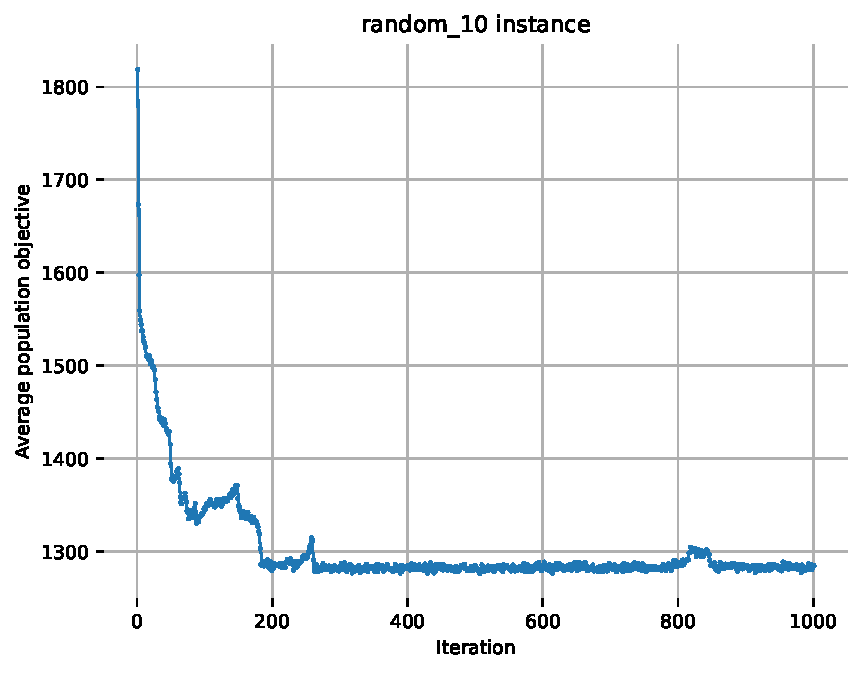
\includegraphics[width=0.8\textwidth]{hyperparameters/max_number_of_iter_random_10}\label{subfig:hyperparams-max-number-of-iter-random-10}}
            \subfloat{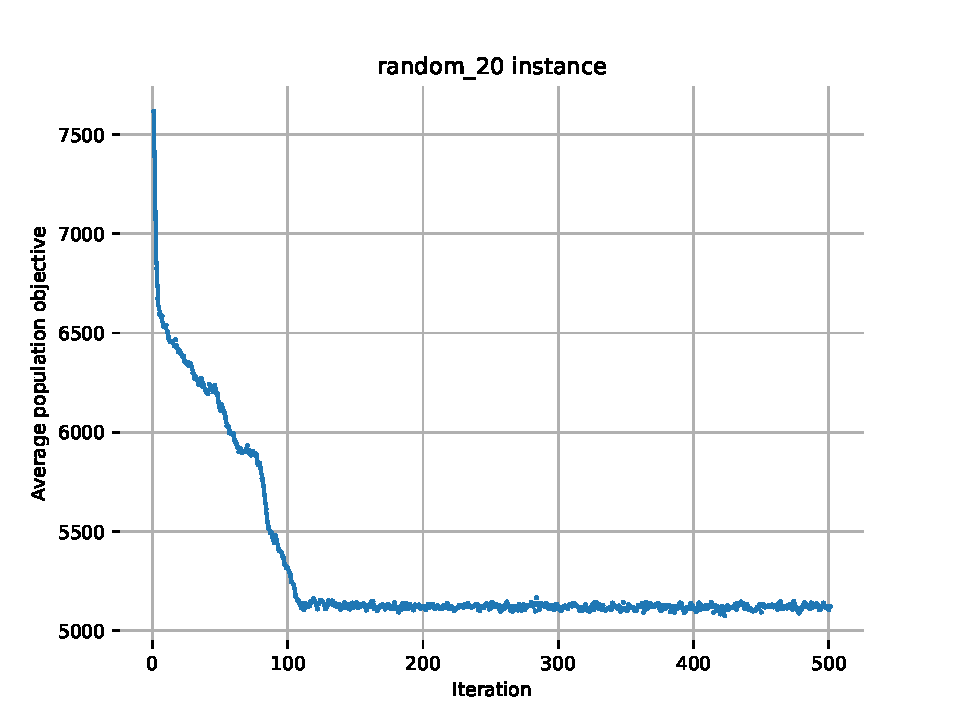
\includegraphics[width=0.8\textwidth]{hyperparameters/max_number_of_iter_random_20}\label{subfig:hyperparams-max-number-of-iter-random-20}}
            \caption[Max number of iter]
            {Testing hyperparameter maximum number of iterations at two random instances.}
            \label{fig:hyperparams-max-number-of-iter}%
        \end{figure}
    \end{landscape}
    \clearpage% Flush page
}